\documentclass[11pt,a4paper]{article}

% ── packages ──────────────────────────────────────────────────────────────────
\usepackage[a4paper, top=20mm, bottom=20mm, left=18mm, right=18mm]{geometry}
\usepackage{tikz}
\usetikzlibrary{shapes.geometric, arrows.meta, positioning, fit, backgrounds,
                automata, calc, decorations.pathreplacing}
\usepackage{booktabs}
\usepackage{array}
\usepackage{enumitem}
\usepackage{xcolor}
\usepackage{listings}
\usepackage{multicol}
\usepackage{titlesec}
\usepackage{fancyhdr}
\usepackage{hyperref}
\usepackage{amsmath}
\usepackage{tabularx}

% ── colours ───────────────────────────────────────────────────────────────────
\definecolor{blk}{HTML}{1A1A2E}
\definecolor{blu}{HTML}{0F3460}
\definecolor{acc}{HTML}{E94560}
\definecolor{grn}{HTML}{16213E}
\definecolor{lgr}{HTML}{A8DADC}
\definecolor{amb}{HTML}{F4A261}
\definecolor{teal}{HTML}{2A9D8F}
\definecolor{pur}{HTML}{6A0572}
\definecolor{lbg}{HTML}{F8F9FA}

% ── page style ────────────────────────────────────────────────────────────────
\pagestyle{fancy}
\fancyhf{}
\fancyhead[L]{\small\textcolor{blu}{\textbf{MC Core — Detailed Reference}}}
\fancyhead[R]{\small\textcolor{acc}{DDR Memory Controller}}
\fancyfoot[C]{\small\thepage}
\renewcommand{\headrulewidth}{0.5pt}

% ── section formatting ────────────────────────────────────────────────────────
\titleformat{\section}
  {\large\bfseries\color{white}}
  {}
  {0em}
  {\colorbox{blu}{\hspace{2pt}\thesection\hspace{6pt}}}[\vspace{-14pt}\textcolor{blu}{\rule{\linewidth}{0.4pt}}]

\titleformat{\subsection}
  {\normalsize\bfseries\color{teal}}
  {\thesubsection}
  {0.5em}
  {}

\titleformat{\subsubsection}
  {\small\bfseries\color{acc}}
  {\thesubsubsection}
  {0.5em}
  {}

% ── list style ────────────────────────────────────────────────────────────────
\setlist[itemize]{itemsep=1pt, topsep=2pt, parsep=0pt}
\setlist[itemize,1]{label=\textcolor{acc}{$\bullet$}}
\setlist[itemize,2]{label=\textcolor{teal}{$\circ$}, leftmargin=1.5em}

% ── TikZ styles ───────────────────────────────────────────────────────────────
\tikzset{
  blk/.style  = {rectangle, rounded corners=3pt, draw=blu, fill=blu!10,
                 minimum width=2.2cm, minimum height=0.7cm,
                 font=\footnotesize\bfseries, align=center, text=blu},
  sub/.style  = {rectangle, rounded corners=2pt, draw=teal, fill=teal!10,
                 minimum width=2cm, minimum height=0.6cm,
                 font=\scriptsize, align=center, text=teal},
  state/.style= {circle, draw=blu, fill=blu!8, minimum size=1.1cm,
                 font=\scriptsize\bfseries, align=center, text=blu},
  arr/.style  = {-Stealth, thick, color=blu},
  rarr/.style = {-Stealth, thick, color=acc},
  tarr/.style = {-Stealth, thick, color=teal},
  grpbox/.style={rectangle, rounded corners=5pt, draw=#1!60, fill=#1!5,
                 dashed, inner sep=6pt},
}

% ══════════════════════════════════════════════════════════════════════════════
\begin{document}

\begin{center}
  {\LARGE\bfseries\color{blu} MC Core — Detailed Reference}\\[4pt]
  {\normalsize\color{teal} Memory Controller Core $\cdot$ Sub-blocks $\cdot$
   FSMs $\cdot$ Timing $\cdot$ Scheduling}\\[2pt]
  {\small\color{gray} DDR2/3/4/5 $|$ LPDDR4/5 $|$ DFI 5.2}
\end{center}
\vspace{-4pt}
\hrule height 1pt
\vspace{6pt}

% ──────────────────────────────────────────────────────────────────────────────
\section{MC Core — Top-Level Block Diagram}
% ──────────────────────────────────────────────────────────────────────────────

\begin{center}
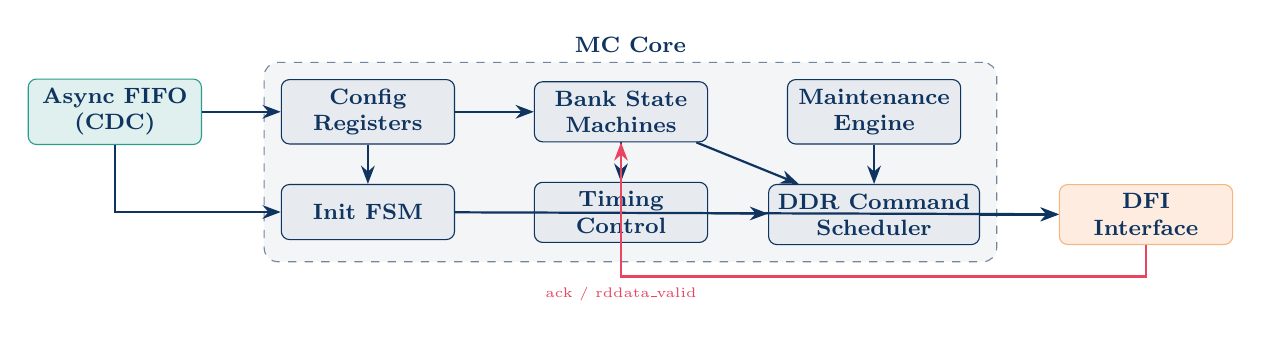
\begin{tikzpicture}[node distance=0.5cm and 0.9cm]

  % ── inputs
  \node[blk, fill=teal!15, draw=teal] (cdc)  {Async FIFO\\(CDC)};

  % ── mc core blocks
  \node[blk, right=1.0cm of cdc]           (cfg)  {Config\\Registers};
  \node[blk, below=0.5cm of cfg]           (init) {Init FSM};
  \node[blk, right=1.0cm of cfg]           (bsm)  {Bank State\\Machines};
  \node[blk, below=0.5cm of bsm]           (tc)   {Timing\\Control};
  \node[blk, right=1.0cm of bsm]           (mnt)  {Maintenance\\Engine};
  \node[blk, below=0.5cm of mnt]           (sch)  {DDR Command\\Scheduler};
  \node[blk, right=1.0cm of sch, fill=amb!20, draw=amb!80] (dfi) {DFI\\Interface};

  % ── arrows
  \draw[arr] (cdc)  -- (cfg);
  \draw[arr] (cdc)  |- (init);
  \draw[arr] (cfg)  -- (bsm);
  \draw[arr] (cfg)  -- (init);
  \draw[arr] (bsm)  -- (tc);
  \draw[arr] (tc)   -- (sch);
  \draw[arr] (bsm)  -- (sch);
  \draw[arr] (mnt)  -- (sch);
  \draw[arr] (init) -- (dfi);
  \draw[arr] (sch)  -- (dfi);

  % ── feedback: DFI→BSM (rddata_valid, ack)
  \draw[rarr] (dfi.south) -- ++(0,-0.4) -| (bsm.south)
    node[midway, below, font=\tiny, color=acc] {ack / rddata\_valid};

  % ── group box
  \begin{scope}[on background layer]
    \node[grpbox=blu, fit=(cfg)(init)(bsm)(tc)(mnt)(sch),
          label={[font=\footnotesize\bfseries\color{blu}]above:MC Core}] {};
  \end{scope}

\end{tikzpicture}
\end{center}

% ──────────────────────────────────────────────────────────────────────────────
\section{Config Registers}
% ──────────────────────────────────────────────────────────────────────────────

\subsection*{Interface}
APB/CSR slave $\rightarrow$ internal register file. Runtime-writable (live
timing update gated by \texttt{ctrl\_idle}).

\subsection*{Key Register Groups}

\begin{center}
\begin{tabularx}{\linewidth}{@{} l l X @{}}
\toprule
\textbf{Group} & \textbf{Width} & \textbf{Contents} \\
\midrule
\texttt{TIMING\_*} & 8--16b each &
  \texttt{tRCD, tCL, tRP, tRAS, tRFC, tRFC2, tFAW, tWR, tRTP,
          tCCD\_L, tCCD\_S, tWTR\_L, tWTR\_S, tRRD\_L, tRRD\_S} \\
\addlinespace
\texttt{MR\_SHADOW[0..6]} & 16b &
  Mirror of DRAM Mode Registers; scheduler reads for MRS cmd emission \\
\addlinespace
\texttt{DDR\_VER} & 3b &
  Selects DDR2/3/4/5 or LPDDR4/5 $\rightarrow$ gates scheduler logic \\
\addlinespace
\texttt{PHY\_OFFSET} & 8b &
  DFI \texttt{dfi\_t\_rddata\_en}, \texttt{dfi\_t\_phy\_wrlat} latency offsets \\
\addlinespace
\texttt{REFRESH\_CFG} & 8b &
  \texttt{tREFI} override, PBR enable (DDR5), 2$\times$ refresh flag \\
\addlinespace
\texttt{ZQCAL\_CFG} & 8b &
  \texttt{tZQCS} interval, ZQCL trigger \\
\addlinespace
\texttt{FREQ\_RATIO} & 2b &
  1:1 / 1:2 / 1:4 $\rightarrow$ \texttt{dfi\_freq\_ratio} to PHY \\
\bottomrule
\end{tabularx}
\end{center}

% ──────────────────────────────────────────────────────────────────────────────
\section{Init FSM}
% ──────────────────────────────────────────────────────────────────────────────

\subsection*{Function}
Power-up sequencing, MRS loading, PHY training handshake.
Emits DFI commands \textbf{directly}, bypassing scheduler.

\vspace{4pt}
\begin{center}
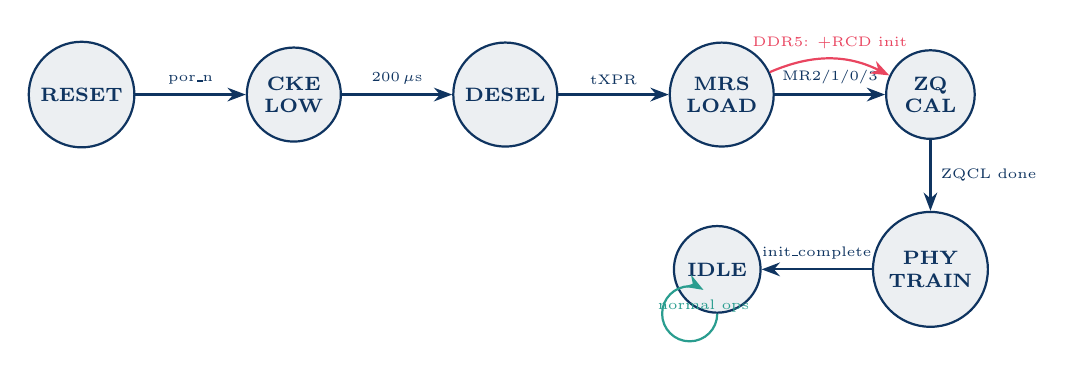
\begin{tikzpicture}[node distance=1.0cm and 1.4cm, -Stealth, thick]

  \node[state]                      (rst)   {RESET};
  \node[state, right=of rst]        (cke)   {CKE\\LOW};
  \node[state, right=of cke]        (desel) {DESEL};
  \node[state, right=of desel]      (mrs)   {MRS\\LOAD};
  \node[state, right=of mrs]        (zq)    {ZQ\\CAL};
  \node[state, below=0.9cm of zq]   (trn)   {PHY\\TRAIN};
  \node[state, left=of trn]         (idle)  {IDLE};

  \draw[arr] (rst)   -- node[above,font=\tiny]{por\_n} (cke);
  \draw[arr] (cke)   -- node[above,font=\tiny]{200\,$\mu$s} (desel);
  \draw[arr] (desel) -- node[above,font=\tiny]{tXPR} (mrs);
  \draw[arr] (mrs)   -- node[above,font=\tiny]{MR2/1/0/3} (zq);
  \draw[arr] (zq)    -- node[right,font=\tiny]{ZQCL done} (trn);
  \draw[arr] (trn)   -- node[above,font=\tiny]{init\_complete} (idle);

  % DDR5 extra
  \draw[rarr, bend left=25] (mrs) to
    node[above,font=\tiny,color=acc]{DDR5: +RCD init} (zq);

  % self loop on IDLE
  \draw[tarr] (idle.south) arc[start angle=0,end angle=-300,radius=0.35]
    node[below,font=\tiny,color=teal]{normal ops};

\end{tikzpicture}
\end{center}

\subsection*{PHY Training Sequence (DFI handshake)}
\begin{itemize}
  \item Assert \texttt{dfi\_init\_start} $\rightarrow$ wait \texttt{dfi\_init\_complete}
  \item Write leveling: toggle \texttt{dfi\_wrlvl\_en}, sample \texttt{dfi\_wrlvl\_strobe}
  \item Gate training: \texttt{dfi\_rdlvl\_gate\_en} / \texttt{dfi\_rdlvl\_resp}
  \item Read DQ training: \texttt{dfi\_rdlvl\_en} / \texttt{dfi\_rdlvl\_resp}
  \item VREF (DDR4/5 / LPDDR5): MRS-based sweep via Init FSM
  \item CA training (LPDDR5): \texttt{dfi\_calvl\_en}
\end{itemize}

% ──────────────────────────────────────────────────────────────────────────────
\section{Bank State Machines}
% ──────────────────────────────────────────────────────────────────────────────

\subsection*{Instantiation}
One FSM per bank $\times$ per rank. DDR4: $4\,\text{ranks} \times 16\,\text{banks}
= 64$ FSM instances. DDR5 with bank groups: $4 \times 2\,\text{BG} \times
4\,\text{banks} = 32$.

\vspace{4pt}
\begin{center}
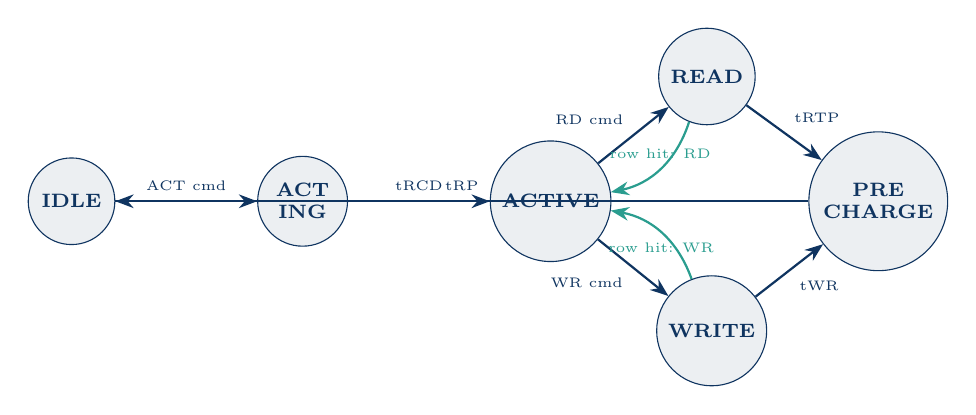
\begin{tikzpicture}[node distance=1.1cm and 1.8cm]

  \node[state]                        (idle) {IDLE};
  \node[state, right=of idle]         (act)  {ACT\\ING};
  \node[state, right=of act]          (actv) {ACTIVE};
  \node[state, above right=0.6cm and 1.0cm of actv] (rd)  {READ};
  \node[state, below right=0.6cm and 1.0cm of actv] (wr)  {WRITE};
  \node[state, right=2.5cm of actv]   (pre)  {PRE\\CHARGE};

  \draw[arr] (idle) -- node[above,font=\tiny]{ACT cmd} (act);
  \draw[arr] (act)  -- node[above,font=\tiny]{tRCD} (actv);
  \draw[arr] (actv) -- node[above left,font=\tiny]{RD cmd} (rd);
  \draw[arr] (actv) -- node[below left,font=\tiny]{WR cmd} (wr);
  \draw[arr] (rd)   -- node[above right,font=\tiny]{tRTP} (pre);
  \draw[arr] (wr)   -- node[below right,font=\tiny]{tWR} (pre);
  \draw[arr] (pre)  -- node[above,font=\tiny]{tRP} (idle);

  % back to ACTIVE on hit
  \draw[tarr, bend left=30] (rd) to
    node[above,font=\tiny,color=teal]{row hit: RD} (actv);
  \draw[tarr, bend right=30] (wr) to
    node[below,font=\tiny,color=teal]{row hit: WR} (actv);

\end{tikzpicture}
\end{center}

\subsection*{Outputs to Scheduler}
\begin{itemize}
  \item \texttt{bank\_available[N]}: bank not precharging / activating
  \item \texttt{open\_row[N][ROW\_W]}: currently active row address
  \item \texttt{row\_hit[N]}: incoming cmd address matches open row
  \item \texttt{bank\_group\_id[N]}: for \texttt{tCCD\_L/S} differentiation
\end{itemize}

% ──────────────────────────────────────────────────────────────────────────────
\section{Timing Control}
% ──────────────────────────────────────────────────────────────────────────────

\subsection*{Architecture}
Per-bank countdown timers, decremented each MC clock.
Output: \texttt{cmd\_legal[N]} vector gating scheduler dispatch.

\begin{center}
\begin{tabularx}{\linewidth}{@{} l l X @{}}
\toprule
\textbf{Timer} & \textbf{Source} & \textbf{Blocks} \\
\midrule
\texttt{tRCD} & ACT issue    & RD/WR to this bank \\
\texttt{tRP}  & PRE issue    & ACT to this bank \\
\texttt{tRAS} & ACT issue    & PRE to this bank (min open time) \\
\texttt{tFAW} & Sliding window & 4-activation gate across all banks (same rank) \\
\texttt{tRFC} & REF issue    & All cmds to rank \\
\texttt{tCCD\_L} & CAS (same BG) & Next CAS same bank group \\
\texttt{tCCD\_S} & CAS (diff BG) & Next CAS different bank group \\
\texttt{tWTR\_L} & WR data end  & RD cmd (same BG) \\
\texttt{tWTR\_S} & WR data end  & RD cmd (diff BG) \\
\texttt{tRTW}    & RD cmd       & WR cmd: $t_{CL} + t_{BL/2} + 2 - t_{CWL}$ \\
\texttt{tRRD\_L/S}& ACT         & Next ACT same/diff BG \\
\texttt{tZQCS}   & ZQCS issue   & All cmds \\
\bottomrule
\end{tabularx}
\end{center}

\subsubsection*{tFAW Sliding Window}
4-entry shift register of ACT timestamps.
$\texttt{faw\_ok} = (\text{now} - \texttt{act\_ts}[3]) \geq t_{FAW}$

% ──────────────────────────────────────────────────────────────────────────────
\section{Maintenance Engine}
% ──────────────────────────────────────────────────────────────────────────────

\subsection{Refresh Manager}

\begin{itemize}
  \item \textbf{Counter}: counts down \texttt{tREFI} (7.8\,$\mu$s DDR4,
        3.9\,$\mu$s at $T > 85^{\circ}$C)
  \item \textbf{Credit accumulation}: up to 8 postponed REFs (JEDEC allows
        burst of 8 back-to-back)
  \item \textbf{Priority escalation}: if credits $\geq$ 8 $\rightarrow$ assert
        \texttt{ref\_urgent} $\rightarrow$ scheduler stalls all others
  \item \textbf{DDR5 PBR}: per-bank refresh — issues
        \texttt{REFpb}\,(bank) instead of \texttt{REFab}
  \item \textbf{LPDDR5}: \texttt{tRFCpb} vs \texttt{tRFCab} selection based on
        \texttt{REFRESH\_CFG[PBR\_EN]}
\end{itemize}

\subsection{ZQ Calibration}

\begin{itemize}
  \item ZQCL: init only / forced via \texttt{ZQCAL\_CFG[ZQCL\_TRIG]};
        stalls all cmds for \texttt{tZQoper}
  \item ZQCS: periodic short calibration every \texttt{tZQCS} interval;
        1 cycle stall only
  \item PHY-side: some DFI implementations expose \texttt{dfi\_calvl\_periodic}
        for automatic PHY ZQ
\end{itemize}

\subsection{Temperature Monitor}

\begin{itemize}
  \item Polls DRAM MR4 (DDR3/4) or MR18 (LPDDR5) via periodic MRR
  \item Thresholds: $T > 85^{\circ}$C $\rightarrow$ \texttt{tREFI} $\div$ 2;
        $T > 95^{\circ}$C $\rightarrow$ derating applied to all timing params
  \item Output: \texttt{derating\_en} $\rightarrow$ Timing Control adds
        derating offsets
\end{itemize}

\subsection{Scrubber (ECC configs)}

\begin{itemize}
  \item Background read patrol: walks full address space at low priority
  \item On ECC error: triggers corrective write-back (\texttt{SEC} correctable)
  \item \texttt{DED} (double-bit) $\rightarrow$ raises \texttt{irq\_ecc\_fatal}
\end{itemize}

% ──────────────────────────────────────────────────────────────────────────────
\section{DDR Command Scheduler}
% ──────────────────────────────────────────────────────────────────────────────

\subsection*{Pipeline Diagram}

\begin{center}
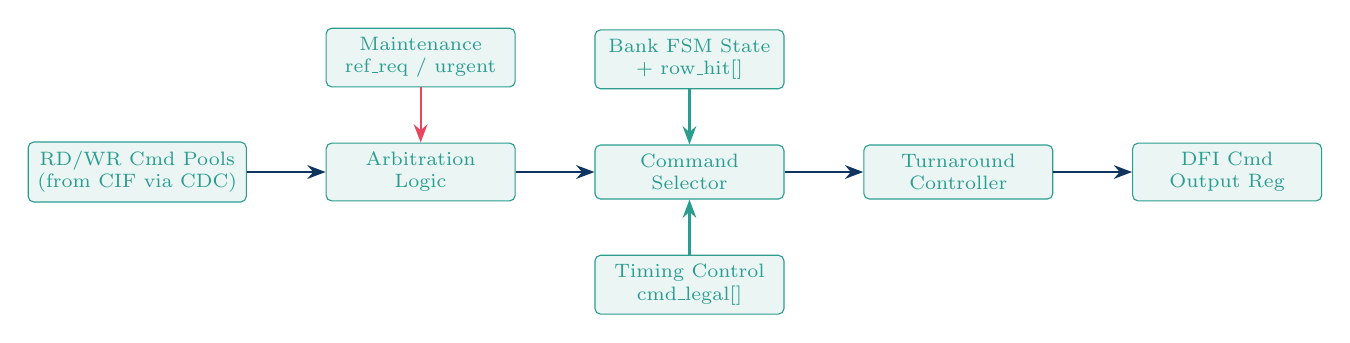
\begin{tikzpicture}[node distance=0.4cm and 1.1cm]

  \node[sub, minimum width=2.4cm] (pool) {RD/WR Cmd Pools\\(from CIF via CDC)};
  \node[sub, right=1.0cm of pool, minimum width=2.4cm] (arb)  {Arbitration\\Logic};
  \node[sub, right=1.0cm of arb,  minimum width=2.4cm] (sel)  {Command\\Selector};
  \node[sub, right=1.0cm of sel,  minimum width=2.4cm] (trn)  {Turnaround\\Controller};
  \node[sub, right=1.0cm of trn,  minimum width=2.4cm] (out)  {DFI Cmd\\Output Reg};

  \draw[arr] (pool) -- (arb);
  \draw[arr] (arb)  -- (sel);
  \draw[arr] (sel)  -- (trn);
  \draw[arr] (trn)  -- (out);

  % inputs from bank FSMs and timing
  \node[sub, above=0.7cm of sel, minimum width=2.4cm] (bsm2) {Bank FSM State\\+ row\_hit[]};
  \node[sub, below=0.7cm of sel, minimum width=2.4cm] (tc2)  {Timing Control\\cmd\_legal[]};
  \draw[tarr] (bsm2) -- (sel);
  \draw[tarr] (tc2)  -- (sel);

  % maintenance
  \node[sub, above=0.7cm of arb, minimum width=2.4cm] (mnt2) {Maintenance\\ref\_req / urgent};
  \draw[rarr] (mnt2) -- (arb);

\end{tikzpicture}
\end{center}

\subsection{Arbitration Logic}

\textbf{Priority order (highest $\rightarrow$ lowest):}
\begin{enumerate}[itemsep=1pt]
  \item Refresh urgent (\texttt{ref\_urgent} asserted)
  \item Refresh nominal (\texttt{ref\_req})
  \item ZQ calibration
  \item Read commands (latency-sensitive)
  \item Write commands
  \item Maintenance (scrubber, MRR)
\end{enumerate}

\textbf{Starvation prevention:}
Age counter per entry. If age $\geq$ \texttt{AGE\_THR} $\rightarrow$ priority
promoted to top of its class.

\subsection{Command Selector}

Selects best legal command from arbitrated pool:

\begin{itemize}
  \item Checks \texttt{bank\_available[N]} AND \texttt{cmd\_legal[N]}
  \item \textbf{Open-page policy (default)}: if \texttt{row\_hit} $\rightarrow$ issue
        CAS directly; skip ACT
  \item \textbf{Closed-page}: force PRE after every access (streaming/random
        workloads)
  \item \textbf{Adaptive}: switch policy based on hit-rate counter threshold
  \item Bank-group scheduling: prefer \texttt{tCCD\_S} path (different BG) for
        back-to-back CAS
\end{itemize}

\subsection{Read/Write Turnaround}

\begin{center}
\begin{tabularx}{\linewidth}{@{} l l X @{}}
\toprule
\textbf{Transition} & \textbf{Constraint} & \textbf{Expression} \\
\midrule
WR $\rightarrow$ RD (same BG) & \texttt{tWTR\_L} &
  $t_{CWL} + t_{BL/2} + t_{WTR\_L}$ \\
WR $\rightarrow$ RD (diff BG) & \texttt{tWTR\_S} &
  $t_{CWL} + t_{BL/2} + t_{WTR\_S}$ \\
RD $\rightarrow$ WR           & \texttt{tRTW}    &
  $t_{CL} + t_{BL/2} + 2 - t_{CWL}$ \\
\bottomrule
\end{tabularx}
\end{center}

DFI pipeline offset applied: \texttt{dfi\_t\_rddata\_en} cycles ahead of CAS for
\texttt{dfi\_rddata\_en}; \texttt{dfi\_t\_phy\_wrlat} for \texttt{dfi\_wrdata\_en}.

\subsection{Output Format (per cycle)}

\begin{center}
\begin{tabularx}{0.9\linewidth}{@{} l l X @{}}
\toprule
\textbf{Field} & \textbf{Width} & \textbf{Meaning} \\
\midrule
\texttt{cmd\_type}  & 3b & ACT / RD / WR / PRE / REF / NOP / MRS / ZQCS \\
\texttt{rank}       & 2b & Target rank \\
\texttt{bank\_group}& 2b & DDR4/5 bank group (0 for DDR3) \\
\texttt{bank}       & 2b & Target bank \\
\texttt{row}        & 17b& Row address (ACT) \\
\texttt{col}        & 11b& Column address (CAS) \\
\texttt{ap}         & 1b & Auto-precharge flag \\
\bottomrule
\end{tabularx}
\end{center}

% ──────────────────────────────────────────────────────────────────────────────
\section{Signal Flow Summary: CIF $\rightarrow$ DFI 5.2}
% ──────────────────────────────────────────────────────────────────────────────

\begin{center}
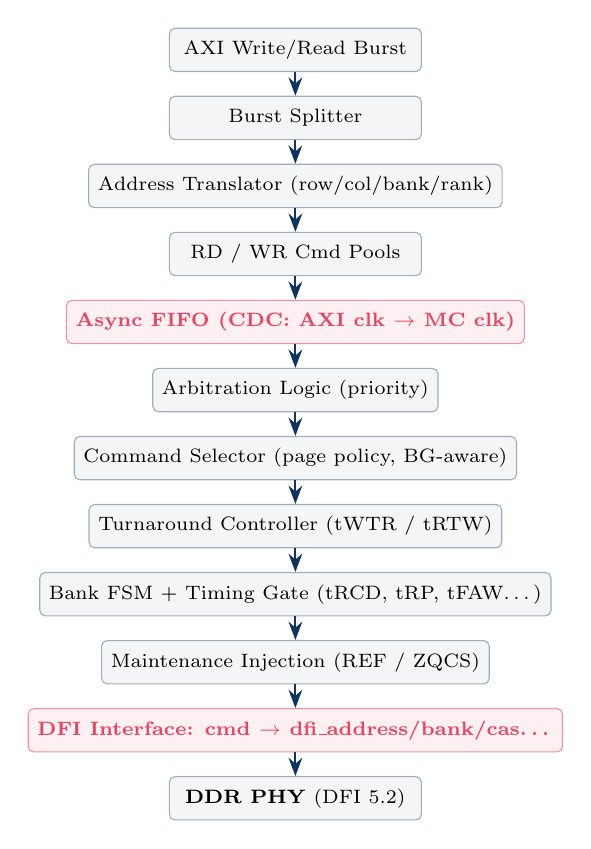
\begin{tikzpicture}[node distance=0.3cm and 0.0cm]
  \tikzset{fl/.style={rectangle, draw=blu!40, fill=blu!5, rounded corners=2pt,
    minimum width=3.2cm, minimum height=0.55cm, font=\scriptsize, align=center}}
  \tikzset{sep/.style={rectangle, draw=acc!60, fill=acc!8, rounded corners=2pt,
    minimum width=3.2cm, minimum height=0.55cm, font=\scriptsize\bfseries,
    text=acc, align=center}}

  \node[fl]  (a1) {AXI Write/Read Burst};
  \node[fl, below=of a1] (a2) {Burst Splitter};
  \node[fl, below=of a2] (a3) {Address Translator (row/col/bank/rank)};
  \node[fl, below=of a3] (a4) {RD / WR Cmd Pools};
  \node[sep, below=of a4] (a5) {Async FIFO (CDC: AXI clk $\to$ MC clk)};
  \node[fl, below=of a5] (a6) {Arbitration Logic (priority)};
  \node[fl, below=of a6] (a7) {Command Selector (page policy, BG-aware)};
  \node[fl, below=of a7] (a8) {Turnaround Controller (tWTR / tRTW)};
  \node[fl, below=of a8] (a9) {Bank FSM + Timing Gate (tRCD, tRP, tFAW\ldots)};
  \node[fl, below=of a9] (a10){Maintenance Injection (REF / ZQCS)};
  \node[sep, below=of a10](a11){DFI Interface: cmd $\to$ dfi\_address/bank/cas\ldots};
  \node[fl, below=of a11] (a12){\textbf{DDR PHY} (DFI 5.2)};

  \foreach \i/\j in {a1/a2, a2/a3, a3/a4, a4/a5, a5/a6, a6/a7,
                     a7/a8, a8/a9, a9/a10, a10/a11, a11/a12}
    \draw[arr] (\i) -- (\j);

\end{tikzpicture}
\end{center}

\vspace{6pt}
\hrule
\vspace{3pt}
{\scriptsize\color{gray}
Reference: JEDEC JESD79-5B (DDR5), JESD209-5B (LPDDR5), MIPI DFI 5.20 spec.
Timing values device-specific; consult datasheet for exact values.}

\end{document}
